\documentclass[tikz,border=0pt]{standalone}
\usepackage{fontspec}
\setmainfont{TeX Gyre Heros}
\setsansfont{TeX Gyre Heros}
\usepackage{amssymb}
\usetikzlibrary{arrows.meta,positioning,calc}
% Shared visual language for Cosmon diagrams. Included after tikz is loaded.
\ifdefined\lightmode
  \definecolor{CosmonBg}{HTML}{E8EFE7}
  \definecolor{CosmonInk}{HTML}{172019}
  \definecolor{CosmonMuted}{HTML}{59665B}
  \definecolor{CosmonFaint}{HTML}{AAB7AA}
  \definecolor{CosmonPanel}{HTML}{F4F7F2}
  \definecolor{CosmonAccent}{HTML}{176D2B}
\else
  \definecolor{CosmonBg}{HTML}{08090C}
  \definecolor{CosmonInk}{HTML}{E7E9E7}
  \definecolor{CosmonMuted}{HTML}{969D97}
  \definecolor{CosmonFaint}{HTML}{444A45}
  \definecolor{CosmonPanel}{HTML}{101317}
  \definecolor{CosmonAccent}{HTML}{3FB950}
\fi

\colorlet{CosmonRoadmap}{CosmonMuted}

\tikzset{
  cosmon text/.style={font=\sffamily\color{CosmonInk}},
  cosmon micro/.style={font=\sffamily\fontsize{6.4}{7.7}\selectfont, text=CosmonMuted},
  cosmon small/.style={font=\sffamily\fontsize{7.4}{9}\selectfont, text=CosmonInk},
  cosmon label/.style={font=\sffamily\bfseries\fontsize{7.2}{8.6}\selectfont, text=CosmonMuted},
  cosmon title/.style={font=\sffamily\bfseries\fontsize{11}{13}\selectfont, text=CosmonInk},
  cosmon frame/.style={draw=CosmonFaint, line width=.55pt, rounded corners=4pt},
  cosmon panel/.style={draw=CosmonFaint, fill=CosmonPanel, line width=.45pt, rounded corners=3pt},
  cosmon molecule/.style={circle, fill=CosmonInk, minimum size=3.6pt, inner sep=0pt},
  cosmon dependency/.style={draw=CosmonMuted, line width=.5pt, -{Latex[length=2.5pt,width=2.1pt]}},
  cosmon data/.style={draw=CosmonInk, line width=1.6pt, {Latex[length=3.1pt,width=2.5pt]}-{Latex[length=3.1pt,width=2.5pt]}},
  cosmon outbound/.style={draw=CosmonAccent, line width=1.05pt, -{Latex[length=3.4pt,width=2.8pt]}},
  cosmon exchange/.style={draw=CosmonInk, line width=.75pt, {Latex[length=3pt,width=2.4pt]}-{Latex[length=3pt,width=2.4pt]}},
  cosmon roadmap/.style={draw=CosmonRoadmap, line width=.65pt, dashed, dash pattern=on 2.4pt off 2.2pt},
  cosmon roadmap arrow/.style={cosmon roadmap, {Latex[length=2.7pt,width=2.2pt]}-{Latex[length=2.7pt,width=2.2pt]}},
  cosmon slot/.style={draw=CosmonAccent, line width=1.2pt, rounded corners=.7pt},
  cosmon peer/.style={circle, draw=CosmonRoadmap, dashed, line width=.6pt, minimum size=13pt, inner sep=0pt},
}

% Canonical glyphs: use these in both diagrams and in the generated legend.
\newcommand{\PilotGlyph}{\textcolor{CosmonAccent}{\ensuremath{\blacklozenge}}}
\newcommand{\MoleculeGlyph}{\textcolor{CosmonInk}{\ensuremath{\bullet}}}
\newcommand{\TraceGlyph}{\textcolor{CosmonAccent}{\ensuremath{\therefore}}}

% The detailed figure's one and only legend, built from the same styles as the art.
\newcommand{\CosmonLegend}{%
  \begin{scope}[shift={(0,0)}]
    \draw[cosmon dependency] (.60,.30) -- (1.22,.30);
    \node[cosmon micro, anchor=west] at (1.36,.30) {thin = ordering dependency};
    \draw[cosmon data] (4.38,.30) -- (5.00,.30);
    \node[cosmon micro, anchor=west] at (5.14,.30) {thick = content in shared files};
    \draw[cosmon roadmap] (8.83,.30) -- (9.45,.30);
    \node[cosmon micro, anchor=west] at (9.59,.30) {dashed = roadmap};
    \node[cosmon micro, anchor=west] at (11.82,.30)
      {\PilotGlyph\ pilot\quad \MoleculeGlyph\ molecule\quad \TraceGlyph\ durable trace};
  \end{scope}%
}


\begin{document}
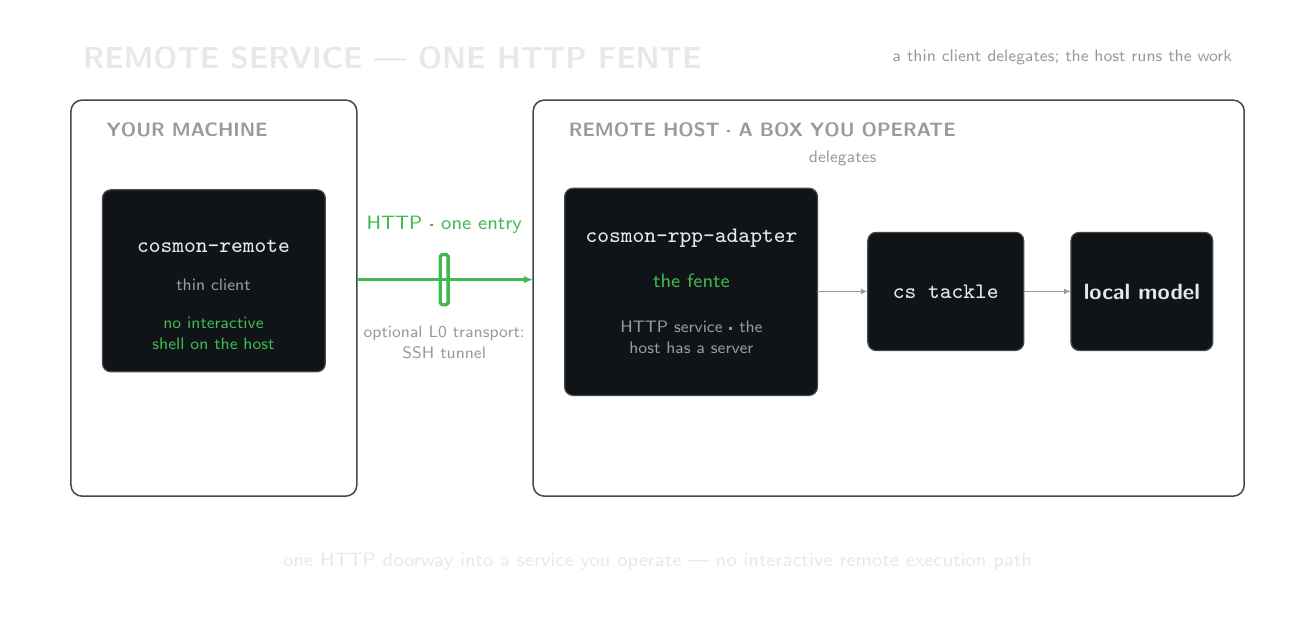
\begin{tikzpicture}[x=1cm,y=1cm]
  \useasboundingbox (0,0) rectangle (16,7.4);
  \node[cosmon title, anchor=west] at (.58,7.02) {REMOTE SERVICE — ONE HTTP FENTE};
  \node[cosmon micro, anchor=east] at (15.42,7.02) {a thin client delegates; the host runs the work};

  % Client machine: intentionally no shell or worker process.
  \draw[cosmon frame] (.55,1.45) rectangle (4.18,6.48);
  \node[cosmon label, anchor=west] at (.88,6.10) {YOUR MACHINE};
  \draw[cosmon panel] (.95,3.03) rectangle (3.78,5.34);
  \node[cosmon small, font=\sffamily\bfseries\fontsize{8.4}{10}\selectfont, align=center]
    at (2.36,4.62) {\texttt{cosmon-remote}};
  \node[cosmon micro, align=center] at (2.36,4.13) {thin client};
  \node[cosmon micro, text=CosmonAccent, align=center, text width=2.25cm]
    at (2.36,3.52) {no interactive shell on the host};

  % The only ingress crosses the machine boundary through the HTTP slot.
  \draw[cosmon outbound] (4.18,4.20) -- (6.42,4.20);
  \draw[cosmon slot] (5.24,3.88) rectangle (5.34,4.52);
  \node[cosmon small, text=CosmonAccent, anchor=south] at (5.29,4.66) {HTTP · one entry};
  \node[cosmon micro, anchor=north, align=center] at (5.29,3.74) {optional L0 transport:\\SSH tunnel};

  % Remote host: service boundary, then the same cs lifecycle and local model.
  \draw[cosmon frame] (6.42,1.45) rectangle (15.45,6.48);
  \node[cosmon label, anchor=west] at (6.75,6.10) {REMOTE HOST · A BOX YOU OPERATE};

  \draw[cosmon panel] (6.82,2.73) rectangle (10.03,5.36);
  \node[cosmon small, font=\sffamily\bfseries\fontsize{8.2}{9.8}\selectfont, align=center]
    at (8.43,4.73) {\texttt{cosmon-rpp-adapter}};
  \node[cosmon small, text=CosmonAccent, align=center] at (8.43,4.18) {the fente};
  \node[cosmon micro, align=center, text width=2.55cm] at (8.43,3.47)
    {HTTP service · the host has a server};

  \draw[cosmon dependency] (10.03,4.05) -- (10.67,4.05);
  \node[cosmon micro, anchor=south] at (10.35,5.52) {delegates};
  \draw[cosmon panel] (10.67,3.30) rectangle (12.65,4.80);
  \node[cosmon small, font=\sffamily\bfseries\fontsize{8.2}{9.8}\selectfont, align=center]
    at (11.66,4.05) {\texttt{cs tackle}};

  \draw[cosmon dependency] (12.65,4.05) -- (13.25,4.05);
  \draw[cosmon panel] (13.25,3.30) rectangle (15.05,4.80);
  \node[cosmon small, font=\sffamily\bfseries\fontsize{8.2}{9.8}\selectfont, align=center]
    at (14.15,4.05) {local model};

  \node[cosmon small, anchor=center, text width=14.8cm, align=center]
    at (8,.62) {one HTTP doorway into a service you operate --- no interactive remote execution path};
\end{tikzpicture}
\end{document}
